\begin{section}*{Assignment 2}
    \begin{subsection}*{Delegation to servers}
        We will use the main application as a means of sending the question data to other
        remote storage servers. The question author will have to submit the question within
        the Question Editor where it will be sent to one of the remote servers via FTP that
        will be initiated by the main server itself. Then the question will get a
        pending status in which it will await approval from an organizer. The moment
        the question gets approved, it will be usable within the application for question
        sets.
    \end{subsection}
    
    \begin{subsection}*{Question Editor}
        We will use one configuration xml file that must have a certain structure. In
        that file the type of the question is determined: multiple choice or regular
        expression. Then it will contain one or more languages that will each contain a
        reference to a question file and feedback file that are both html files. There
        will also be one or more answer elements for multiple choice questions with one
        of them marked as correct and a regular expression for the other type.
        
        This is how the questions will be created internally. There will also be an extra
        layer above that, the Question Editor.
        Question authors and organizers are the only ones who have access to this
        sub-application. There they can create a new question from scratch and organizers
        can also edit an existing question that is already available in the database.
        
        When they create a new question they will see Figure~\ref{qe-index} where they
        must first select the question type:
        multiple choice or open answer. After that they will see a screen similar to the
        one in Figure~\ref{qe-question}. There they can add languages for the question; they must add at
        least one. The languages will act as tabs for the editor, and at all times they
        can add and remove languages. For each language they can add answers with
        one marked as the correct one for multiple choice questions like in Figure~\ref{qe-answers}.
        For the other type they can enter a required input answer. Advanced users can also
        enter Java-accepted regular expressions. They can also edit the question and feedback html file
        with a simple WYSIWYG editor that is also capable of entering images. Uploading
        files will be as simple as dragging files to your browser like in Figure~\ref{qe-upload}.
        When they are ready, they can push on the 'submit' button on which the application
        will validate the question and notify the author for mistakes. Like for example
        not marking one of the possible answers as correct.
        
        Advanced users still have the option to download the question packs and manually
        edit them and import them to the question editor.
        
        Organizers are always capable of previewing existing questions from within the
        application.
        
        \begin{figure}[h!]
            \caption{Index page of the question editor.}
            \centering
            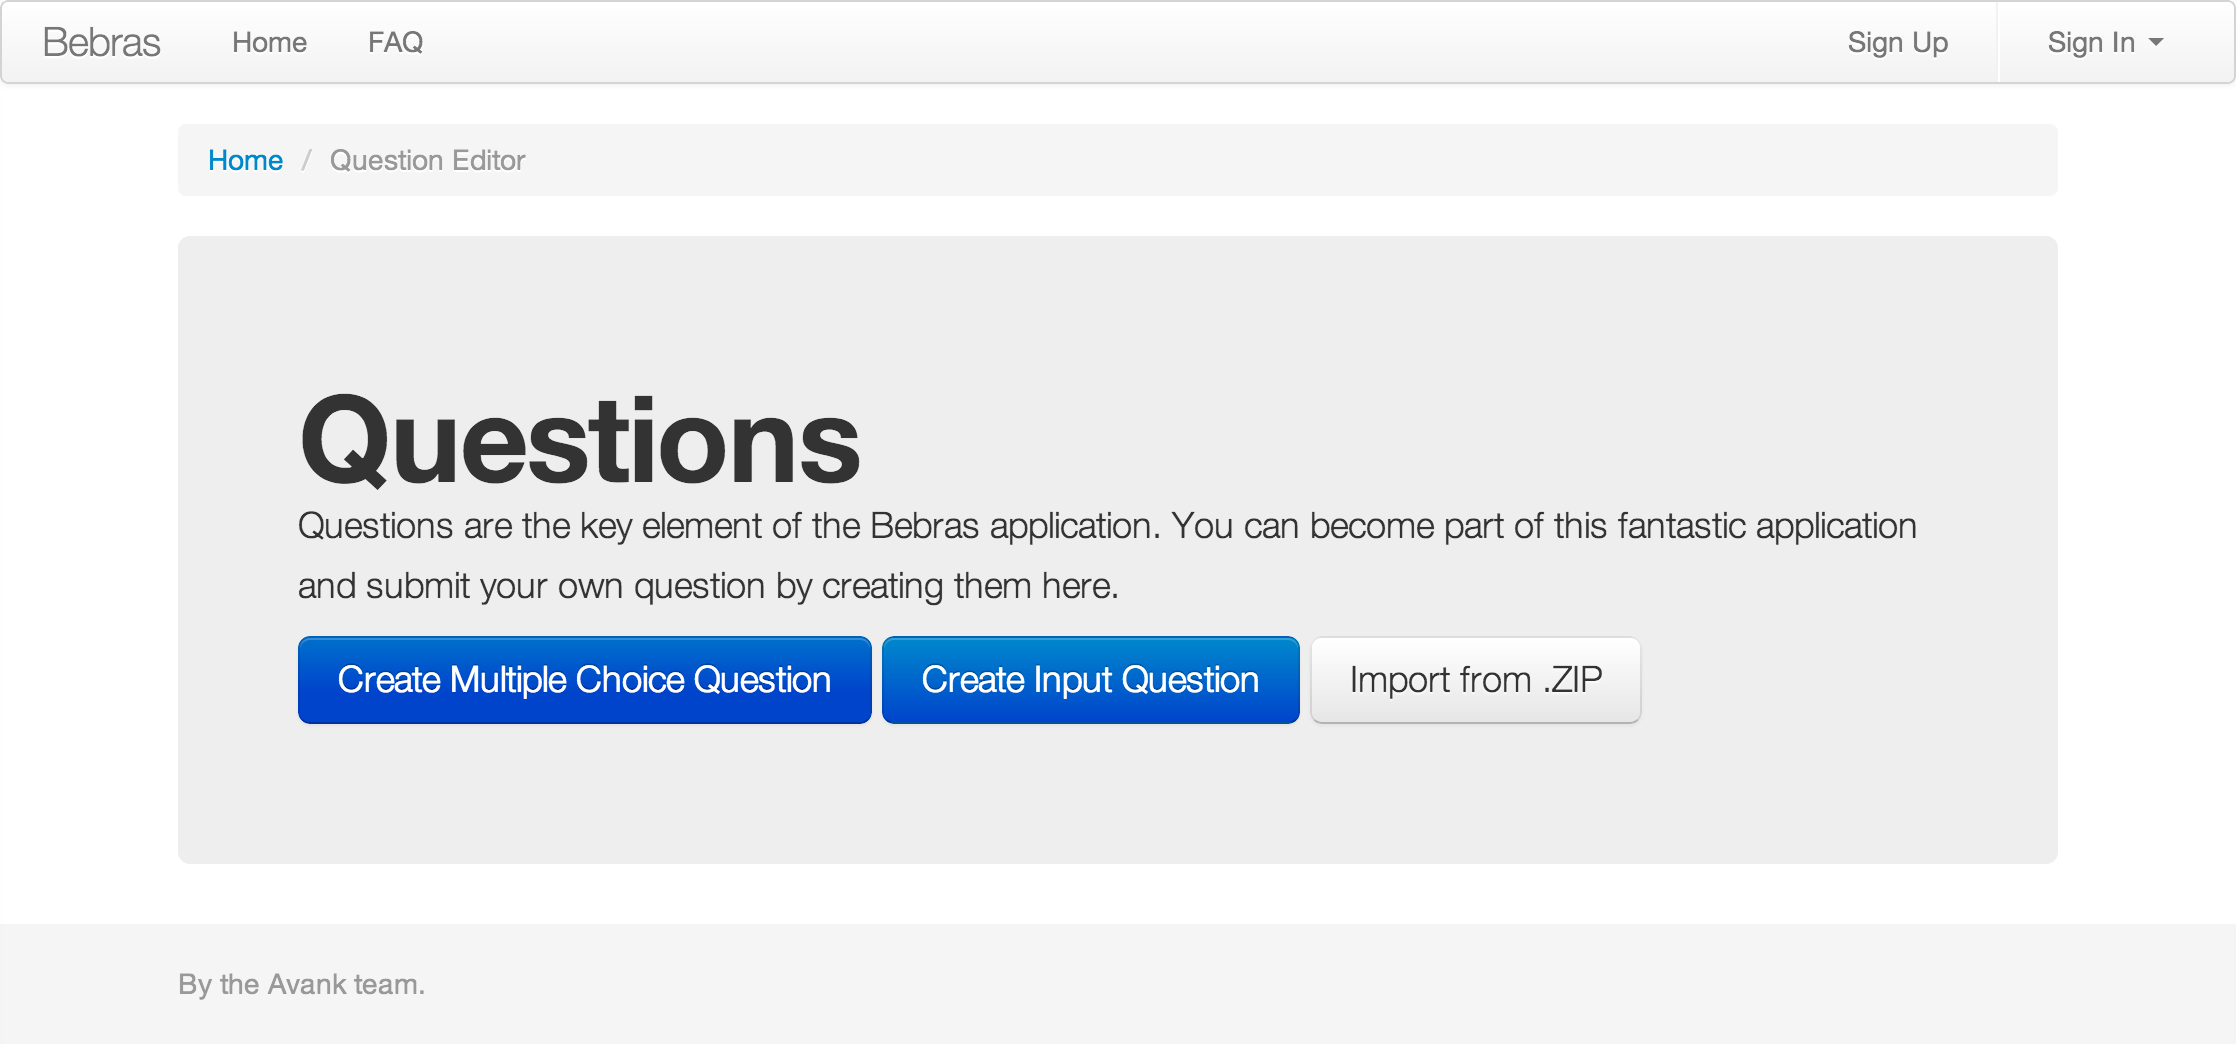
\includegraphics[width=1\textwidth]{img/index}
            \label{qe-index}
        \end{figure}
        
        \begin{figure}[h!]
            \caption{Type in a question in a nice WYSIWYG editor.}
            \centering
            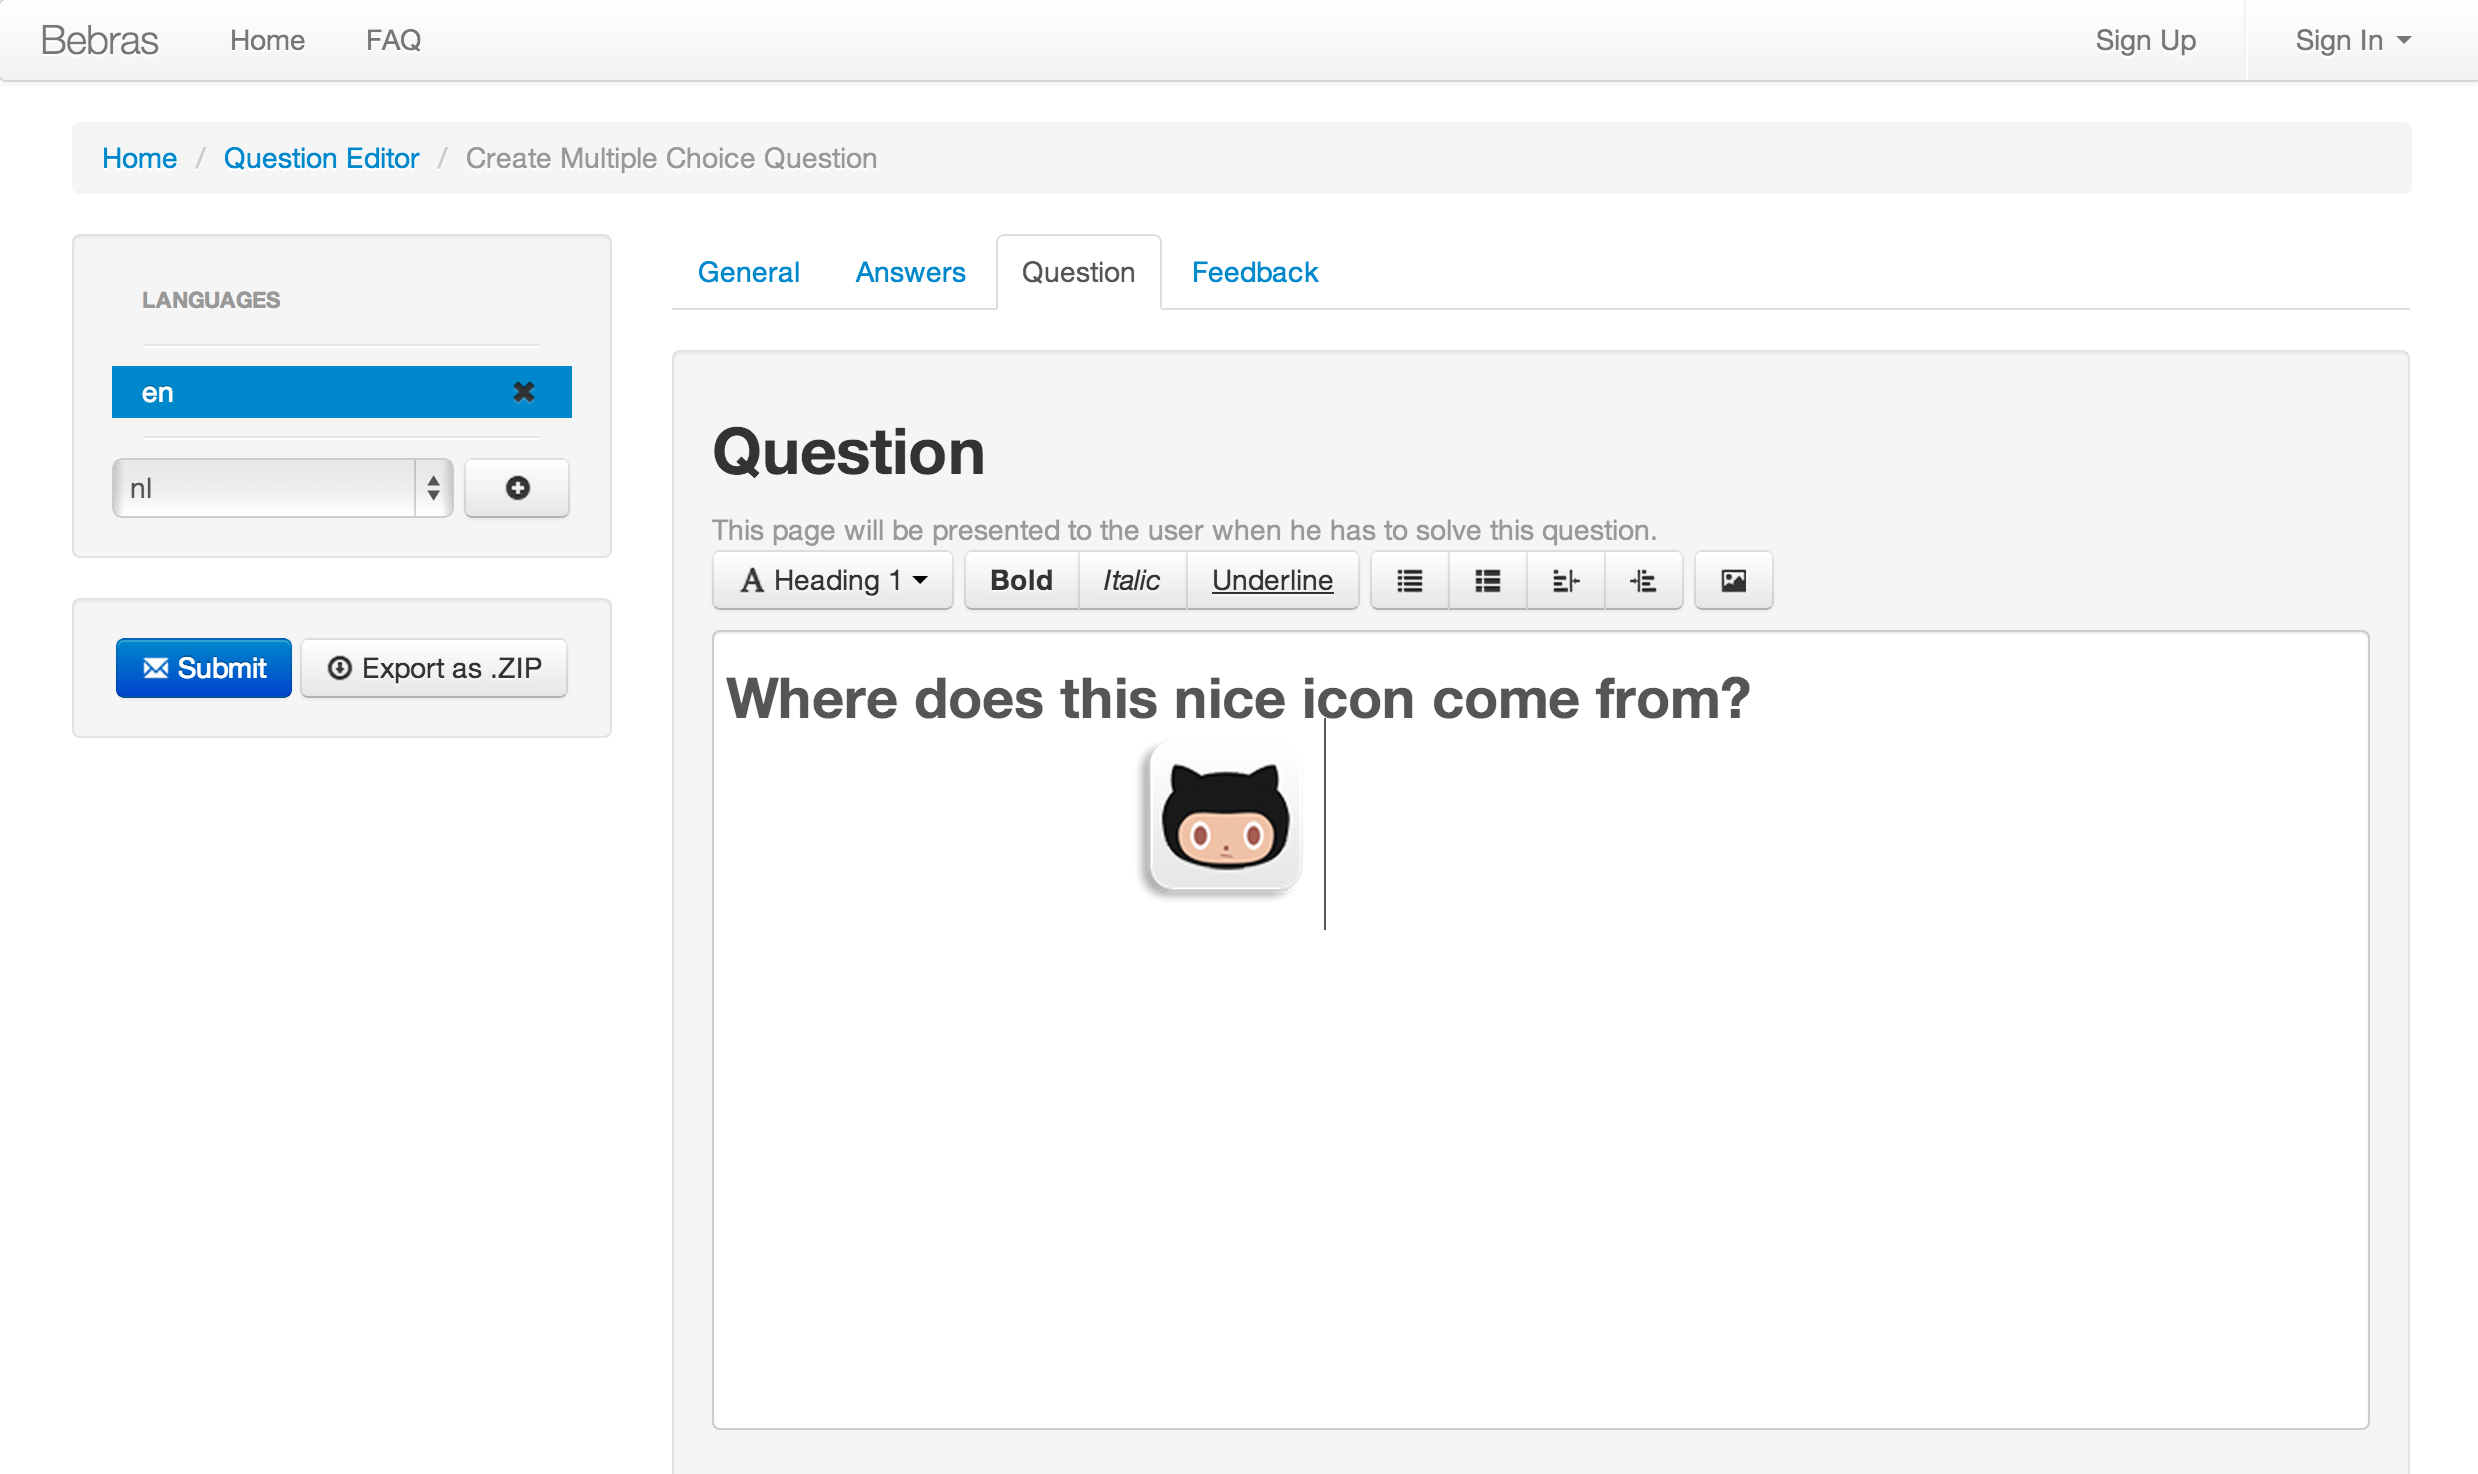
\includegraphics[width=1\textwidth]{img/question}
            \label{qe-question}
        \end{figure}
        
        \begin{figure}[h!]
            \caption{Upload images that can be added inside the question and/or feedback.}
            \centering
            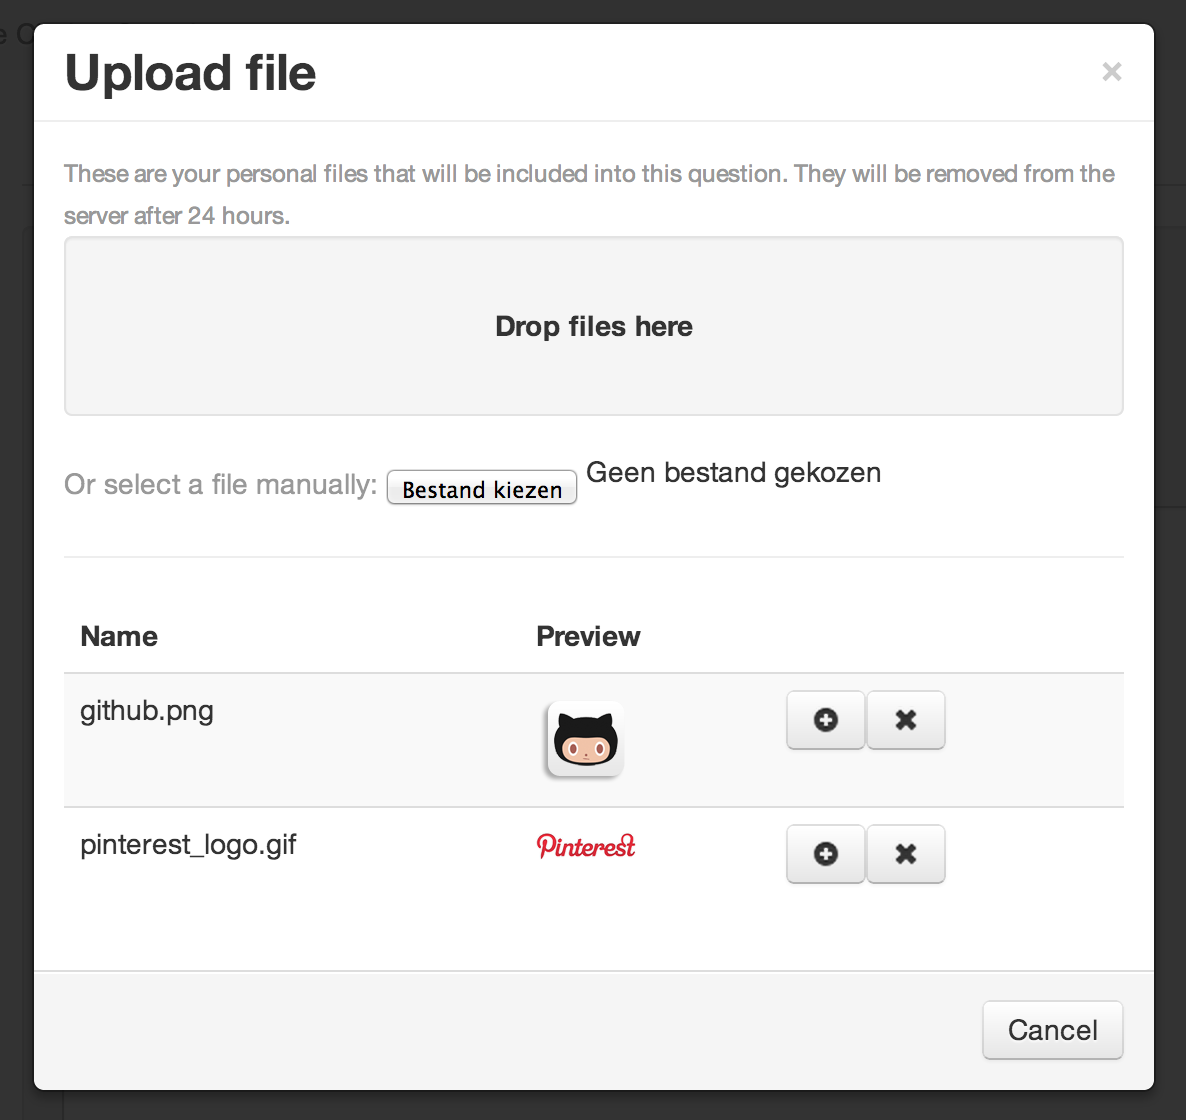
\includegraphics[width=1\textwidth]{img/upload}
            \label{qe-upload}
        \end{figure}
        
        \begin{figure}[h!]
            \caption{Add possible answers for multiple choice questions.}
            \centering
            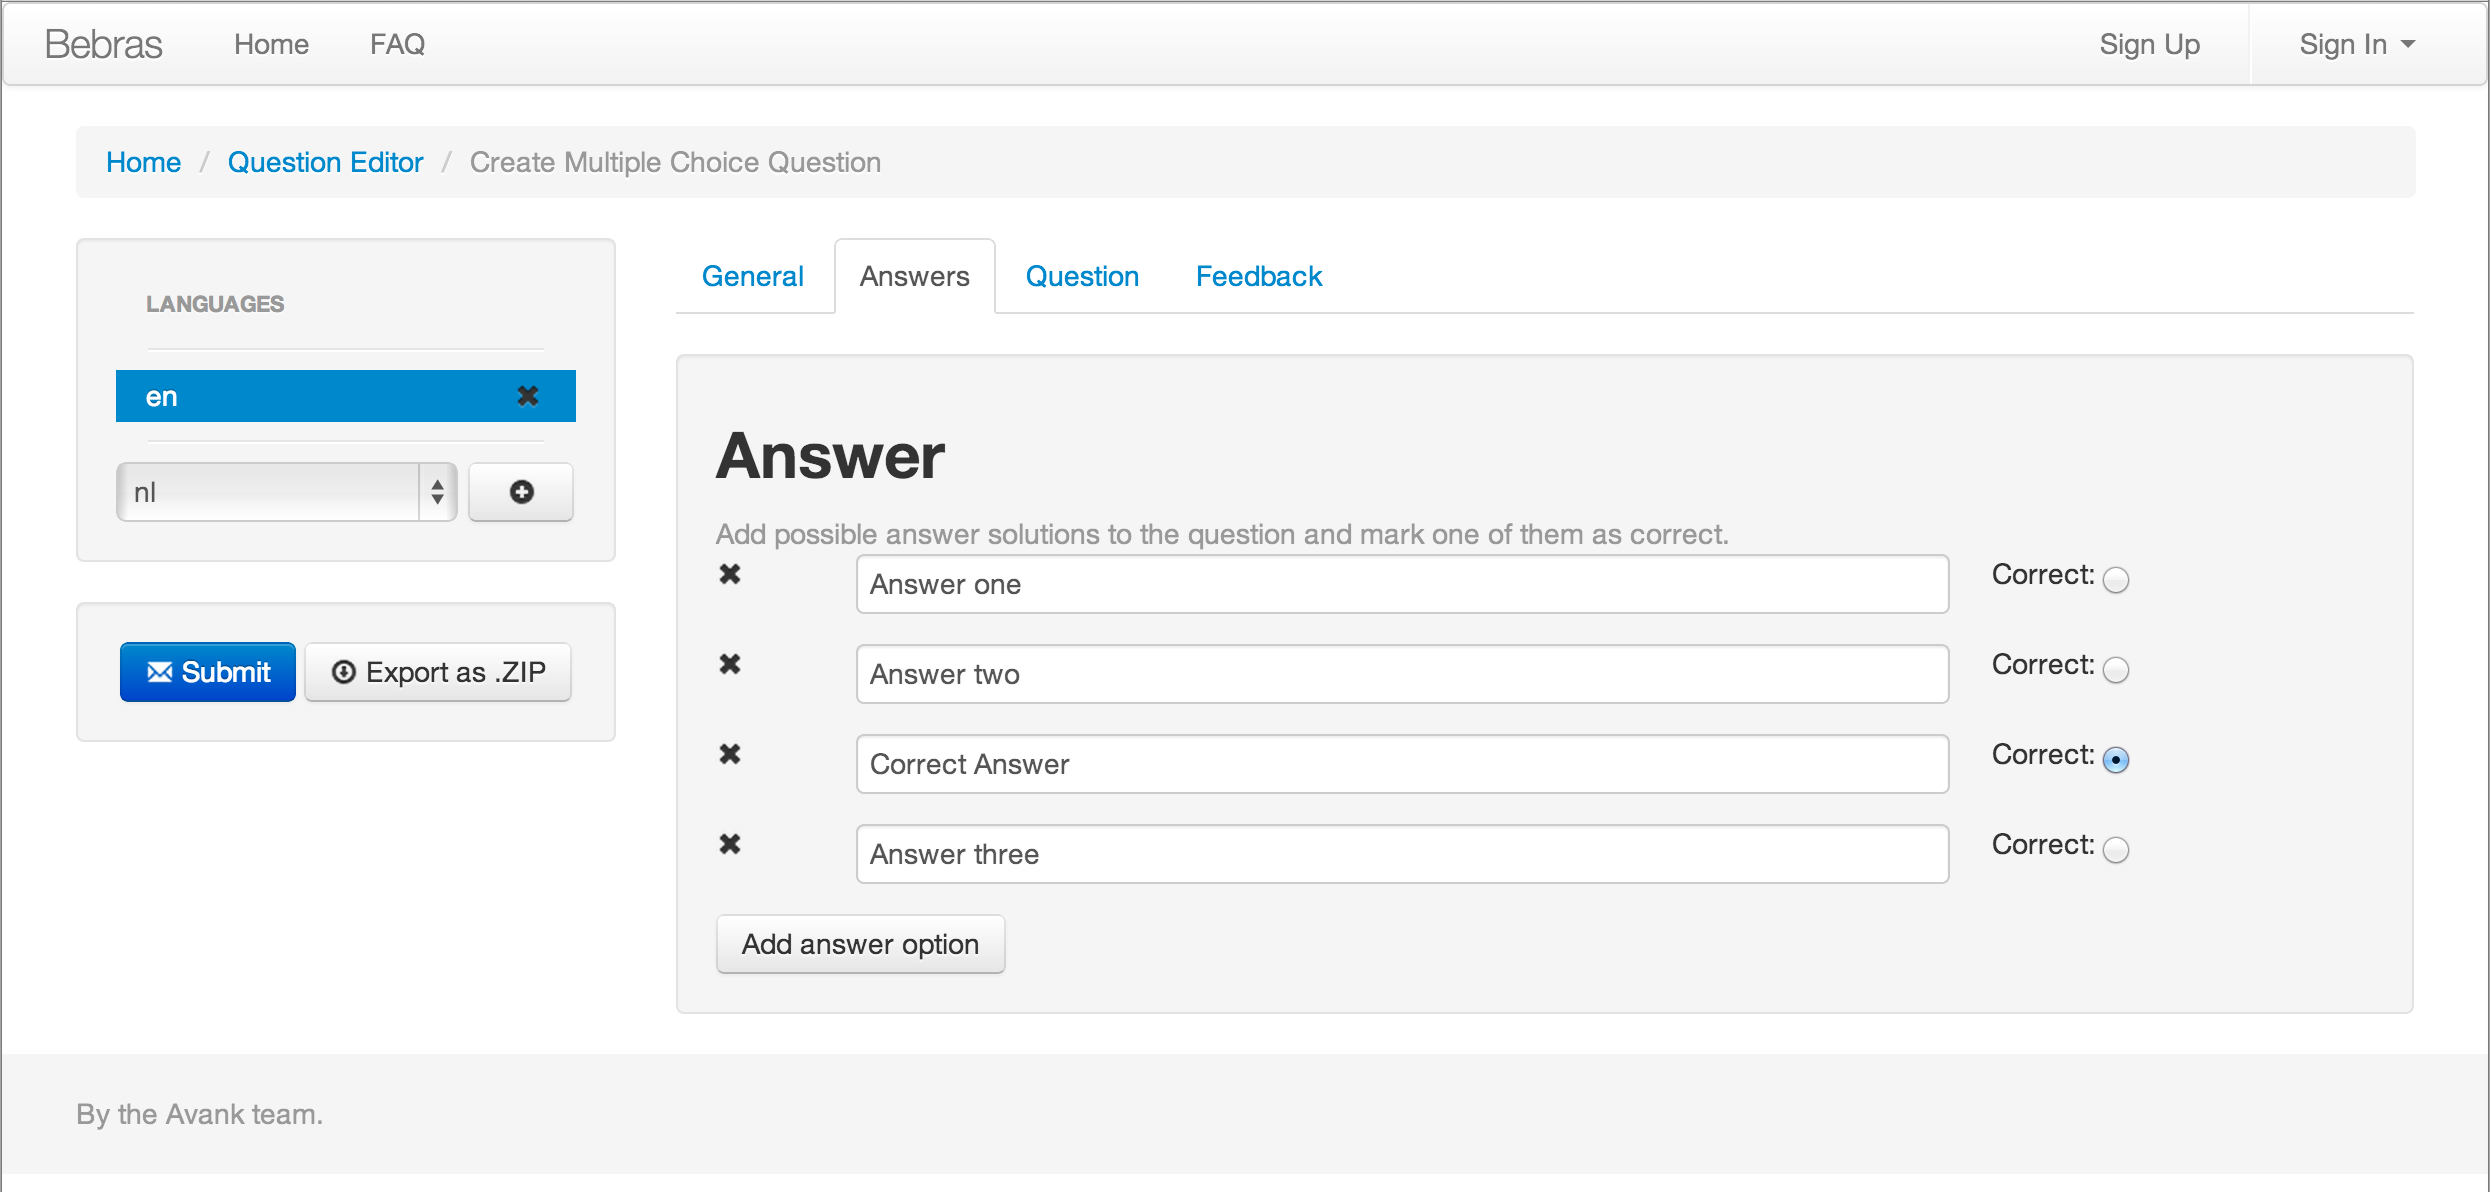
\includegraphics[width=1\textwidth]{img/answers}
            \label{qe-answers}
        \end{figure}
    \end{subsection}  
\end{section}